% !TeX root = main.tex
% Mirror: https://github.com/SIGma-UIUC/presentation-format
% --------------------------------------------------------------------
% This is a simple Beamer document. Its shared styles live in ../sty/.
% Reading the comments should help you create a presentation even if
% you've never used Beamer before.
% --------------------------------------------------------------------

% Set our document class to Beamer
% Add handout option to collapse pauses for printing
\documentclass[aspectratio=169, handout]{beamer}

% Presentation mechanics, then the SIGma look on top of them
\usepackage{../sty/slides}
\usepackage{../sty/sigma/sigma}

% Maths macros and algorithm environments
\usepackage{../sty/math}
\usepackage{../sty/stat}
\usepackage{../sty/algo}
\usepackage{../sty/code}

\usepackage{tikz}
\usetikzlibrary{graphs}
\usetikzlibrary{arrows.meta}

\usepackage{pdfpages}

% Set a title
\title{SIGma Fall 2026}

% Set a subtitle if you desire
\subtitle{CG:SHOP Work Session}

% Whoever worked on the presentation:
\author{Mihir Tandon}

% Date looks ugly, so leave blank
\date{}

% An institute name, if you're so inclined
% \institute{University of Illinois Urbana-Champaign}
% --------------------------------------------------------------------

% Begin document
\begin{document}

% Beamer calls each slide a "frame", defined within the environment:
% \begin{frame}
%   <frame content here>
% \end{frame}

% This frame is just the title.
\begin{frame}
    \titlepage
\end{frame}

% A frame with the table of contents.
% This frame's title is "Outline".
\begin{frame}{Outline}
    \tableofcontents
\end{frame}

\section{CG:SHOP}
\frame{\sectionpage}

\begin{frame}{What is CG:SHOP?}
    \begin{itemize}
        \item \textbf{CG:SHOP} (Computational Geometry: Solving Hard Optimization Problems) is a computational geometry competition for students and researchers.
        \item Each year, teams build solvers for a difficult geometric optimization problem.
        \item The 2027 challenge is \textbf{Multi-Robot Lawn Mowing for Polyominoes}.
    \end{itemize}

    \vspace{0.3cm}
    \centering
    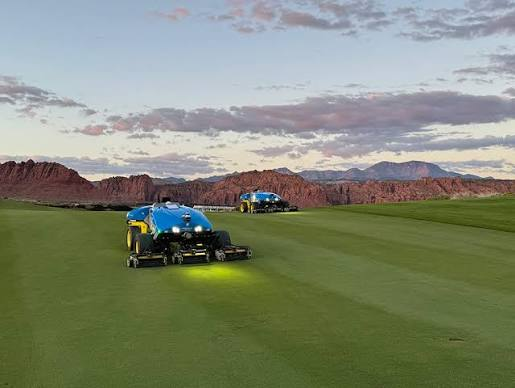
\includegraphics[width=0.42\textwidth]{images/lawn-mower.png}
\end{frame}

\begin{frame}{Problem Background}
    \begin{itemize}
        \item A \textit{polyomino} is a polygonal region made from grid cells whose boundary is horizontal and vertical.
        \item Each problem instance gives us a region $R$ (the \emph{field}), a cutter shape $K$, a center point $c \in K$, and a number of cutters $C$, where $R$ and $K$ are polyominoes.
        \item Each cutter moves its center along a closed, axis-parallel trajectory (will define later).
        \item Cutters do not block one another and may leave $R$.
        \item \textit{Problem Statement}: Given a \emph{field} $R$ and $C$ cutters with fixed shape, find a list of trajectories $T_1,T_2,\ldots,T_C$ that cover the entire field, while minimizing the length of the longest trajectory.
    \end{itemize}
\end{frame}
\begin{frame}{An Example}
    \centering
    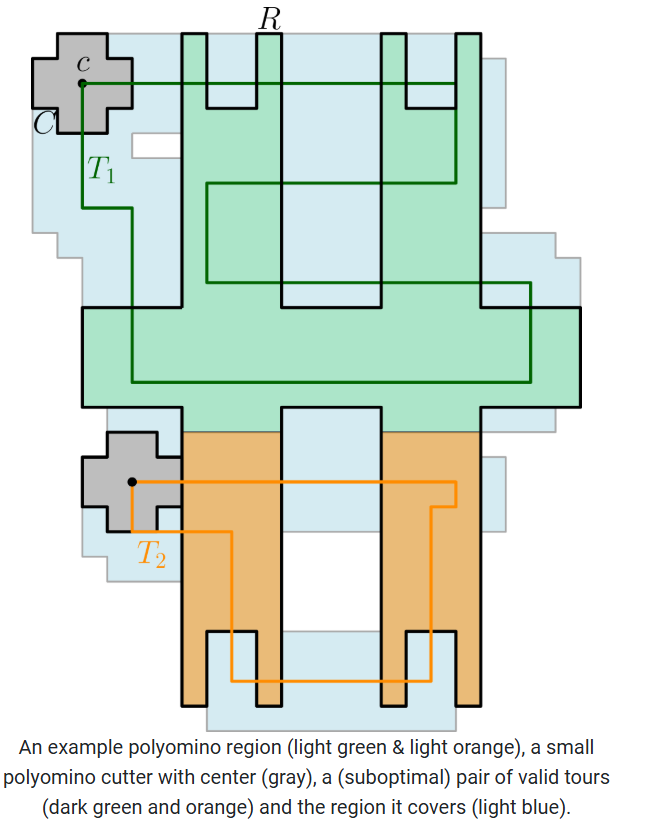
\includegraphics[height=0.78\textheight, keepaspectratio]{images/polyomino.png}
\end{frame}
\begin{frame}{Formal Problem Statement}
    \begin{itemize}
        \item \textbf{Input:} a polyomino region $R$, a cutter shape $K$ with center $c$, and an integer $C$.
        \item \textbf{Solution:} exactly $C$ closed trajectories $T_1, \dots, T_C$ for the cutter centers.
        \item A trajectory is a cyclic sequence of points
              $T_i = (p_{i,0}, \dots, p_{i,m_i - 1})$ with
              $p_{i,j} \in \mathbb{Z}^2$ and axis-parallel edges.
        \item Its length is
              \[
                  \ell(T_i) =
                  \sum_{j = 0}^{m_i - 1}
                  \norm{p_{i,j+1} - p_{i,j}},
                  \qquad p_{i,m_i} = p_{i,0}.
              \]
        \item We require that every cell of $R$ is swept by at least one translated cutter.
        \item \textbf{Objective:} minimize $\max_i \ell(T_i)$.
        \item Note: In case you were wondering, this is NP-hard.
    \end{itemize}
\end{frame}

\begin{frame}{CG:SHOP Logistics}
    \begin{itemize}
        \item The competition starts on October 15, 2026.
        \item Final submissions are due January 31, 2027.
        \item Example instances and Python utilities are already available.
        \item Discord for CG:SHOP problems: \href{https://discord.gg/3FXC6xzzWe}{discord.gg/3FXC6xzzWe}.
        \item We might also have a professor advise us, this is still TBD.
    \end{itemize}

    \vspace{0.2cm}
    \centering
    
\includegraphics[width=0.25\textwidth]{images/qr-code-cgshop.png}
\end{frame}

\begin{frame}{CG:SHOP Logistics}
    \begin{itemize}
        \item Please start taking a look at the \href{https://cgshop.ibr.cs.tu-bs.de/competition/cg-shop-2027/}{challenge website}.
        \begin{itemize}
            \item There are also many papers out there about similar problems.
        \end{itemize}
        \item We will split into \textit{algorithm} and \textit{implementation} teams.
        \begin{itemize}
            \item \textit{Algorithm} teams will work on reading/understanding existing literature and generating/doing basic testing of potential algorithms.
            \item \textit{Implementation} teams will work on implementing the algorithms from the algorithm team as well as modifying existing algorithms.
            \item Both teams need a strong understanding of current research in this area.
        \end{itemize}
        \item Bring questions, observations, or solver ideas to the next meeting.
    \end{itemize}
\end{frame}

\begin{frame}{Project AI Policy}
    \begin{itemize}
        \item You are free to use AI for understanding papers, setting up environments, or generating algorithmic ideas, but treat its output with caution.
        \item We will not be merging any code that we do not understand or is clearly AI-generated.
              \begin{itemize}
                  \item We need to understand the code that we write.
              \end{itemize}
    \end{itemize}
\end{frame}

\section{Git/Env Setup}
\frame{\sectionpage}

\end{document}
